I dette afsnit findes dokumentation for projektets Data Access Layer. Klassediagrammet for hele komponenten på figur~\ref{fig:databaseFullClass} i Appendix~\ref{app:figs} på side~\pageref{fig:databaseFullClass}.

\section{Klassebeskrivelser}
 
\subsection{DatabaseContext}
DbContext er en del af Entity Frameworket. Som det kan ses på figur~\ref{fig:dbContextClass} arver DatabaseContext fra DbContext \cite{microsoftdbcontext} og udgør da bindeleddet fra koden til databasen.

\begin{figure}
\centering
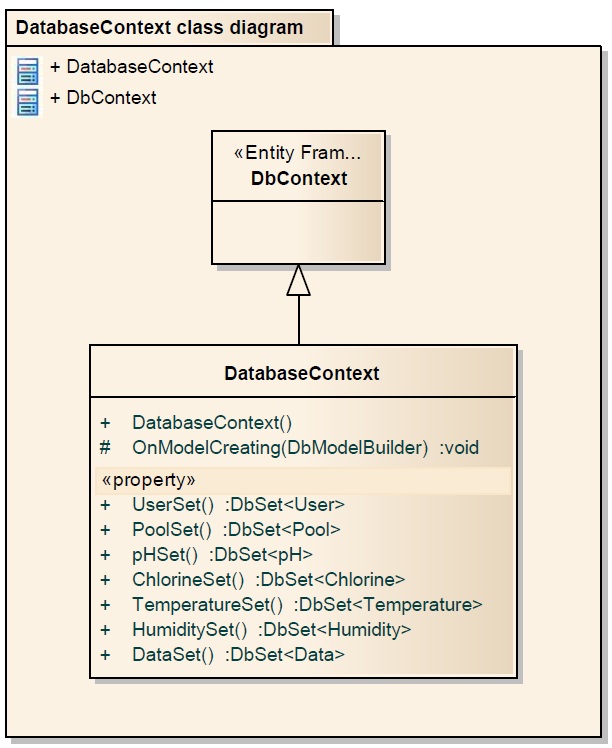
\includegraphics[width=0.5\linewidth]{figs/implementering/dbContextClass.PNG}
\caption{Klassen DatabaseContext.}
\label{fig:dbContextClass}
\end{figure}

Entities er defineret i klassen som \textit{public virtual DbSet<T>} hvor typen er den specifikke entity.
DatabaseContext objektet skal oprettes når der laves en query på databasen eller sættes data ind.
På en DbSet property kan der kaldes Add(), som tilføjer en entity i den kontekst der kaldes i. Herefter skal DbContext’s SaveChanges() metode kaldes for at ændringerne skrives i databasen.

\subsection{SmartpoolDB}
SmartpoolDB implementerer ISmartPoolDB og står for at initialisere DataAccess, UserAccess og PoolAccess gennem deres interfaces. SmartpoolDB kan da bruge af klienter når data access funktionalitet skal bruges. I SmartpoolDB klassen findes også administratormetode der står for at slette hele databasen.Klassen \textit{SmartpoolDB} kan ses på figur~\ref{fig:smartpoolDBClass}

\begin{figure}
\centering
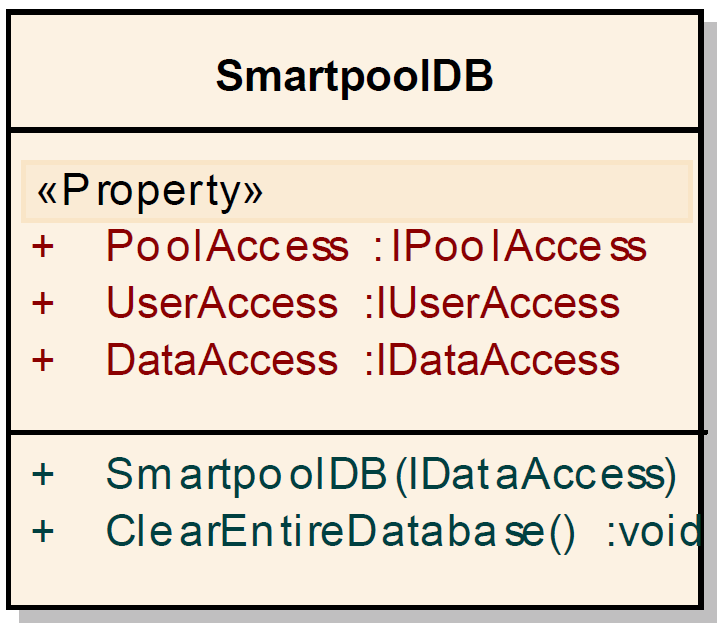
\includegraphics[width=0.3\linewidth]{figs/implementering/smartpoolDBClass.PNG}
\caption{Klassen SmartpoolDB}
\label{fig:smartpoolDBClass}
\end{figure}

\subsubsection{Constructor}\

\textit{public SmartpoolDB(IDataAccess dataAccess)}

Constructoren stå udelukkende for at initialisere SmartpoolDB-klassens pool, user- og dataaccess properties.

\subsubsection{ClearEntireDatabase}\

\textit{public void ClearEntireDatabase()}

Metoden kalder DeleteAll metoderne på dens egen properties, og derved fjernes alt data i databasen.

\subsubsection{Properties}

\begin{itemize}
	\item \textit{public IPoolAccess PoolAccess { get; }}
	\item \textit{public IUserAccess UserAccess { get; }}
	\item \textit{public IDataAccess DataAccess { get; }}
\end{itemize}

\subsubsection{Klassen UserAccess}
Klassen UserAccess implementerer IUserAccess og står for at skrive og læse user records til/fra databasen.
UserAccess indeholer administrator funktionalitet til at slette alle users på databasen. Herudover står UserAccess for data editing af users samt validering af userdata før det gemmes.

\begin{figure}[h]
\centering
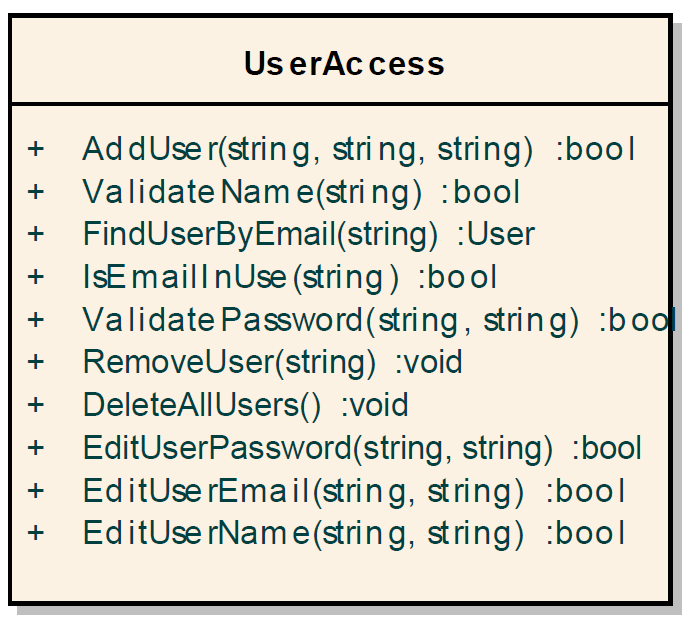
\includegraphics[width=0.4\linewidth]{figs/implementering/UserAccessClass.PNG}
\caption{Klassen UserAccess}
\label{fig:UserAccessClass}
\end{figure}


\paragraph{Metodebeskrivelser}
I dette afsnit findes metodebeskrivelser for klassen \textit{UserAccess}.

\subparagraph{AddUser}\

\textit{bool AddUser(string fullname, string email, string password)}

Står for at indsætte en user i databasen. Metoden kalder IsEmailInUse samt ValidateName før der oprettes et database kontekst objekt af typen DataBaseContext. På Kontekstobjektets DbSet<User> property kaldes Add metoden med den nye User som parameter. Herefter gemmes den nye User i databasen ved at kalde SaveChanges metoden på kontekstobjektet. AddUser returnerer false hvis der er fejl i enten check på email eller fullname. Hvis det lykkes at tilføje brugeren til databasen returneres true. Se metodens sekvensdiagram på figur~\ref{fig:adduser}

\begin{figure}[h]
\centering
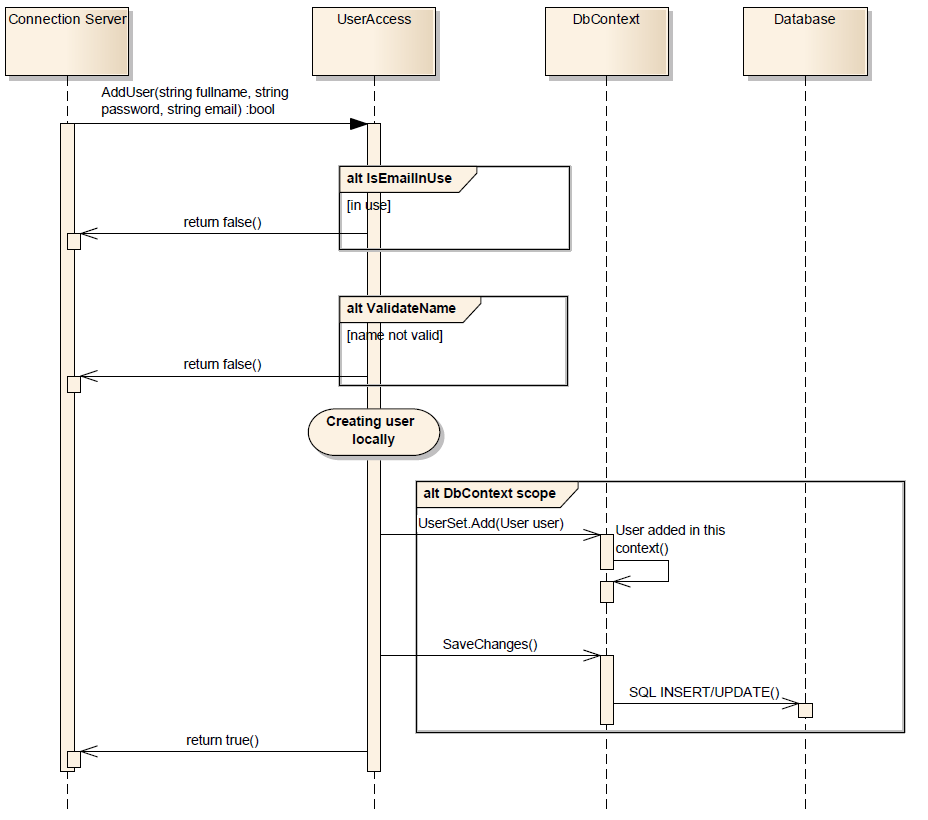
\includegraphics[width=\linewidth]{figs/dbSeq/adduser.PNG}
\caption{Sekvensdiagram for Metoden AddUser}
\label{fig:adduser}
\end{figure}


\subparagraph{FindUserByEmail}\

\textit{User FindUserByEmail(string email)}

Søger i databasen efter en User med den email der angives som parameter. Det må ikke eksistere flere brugere med samme email i databasen. Søgningen udføres med et LINQ statement på databasekonteksten. Se kodeudsnit~\ref{code:finduser}. Metoden returnerer den fundne User, med mindre der kastes en exception.
Se metodens sekvensdiagram på figur~\ref{fig:findUserByEmail}.

\begin{lstlisting}[caption=Kodeudsnit fra metoden FindUserByEmail, label=code:finduser]
...
using (var db = new DatabaseContext())
{
	var searchByEmail = from search in db.UserSet
			where search.Email.Equals(email)
			select search;

	if (searchByEmail.Count() > 1) throw new    	MultipleOccourencesOfEmailWasFoundException();
	if (searchByEmail.Count() == 0) throw new UserNotFoundException();

	foundUser = searchByEmail.First();
}
...	
\end{lstlisting}


\begin{itemize}
	\item \textit{MultipleOccourencesOfEmailWasFoundException()} - Sikkerhedsforanstaltning ved forekomst af flere ens emails.
	\item \textit{UserNotFoundException()} - Kastes hvis der ikke findes en bruger med den angivne email addresse i databasen.
\end{itemize}

\begin{figure}[h]
\centering
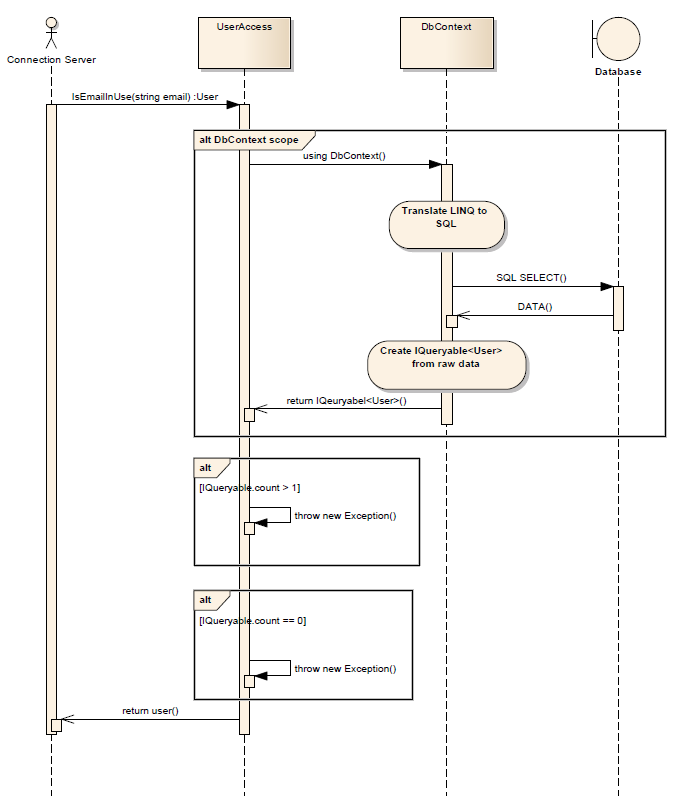
\includegraphics[width=\linewidth]{figs/dbSeq/findUserByEmail.PNG}
\caption{Sekvensdiagram for metoden FindUserByEmail}
\label{fig:findUserByEmail}
\end{figure}


\subparagraph{IsEmailInUse}\

\textit{bool IsEmailInUse(string email)}

Laver en LINQ query på databasekontekst objektet og checker om der findes en mailadresse i databasen der matcher, den som er givet med som parameter. Metoden returnerer false hvis mailaddressen ikke er i brug, og true hvis den er.

I sekvensdiagrammet på figur~\ref{fig:isEmailInUse}, kan det se hvordan en email checkes.

\begin{figure}[h]
\centering
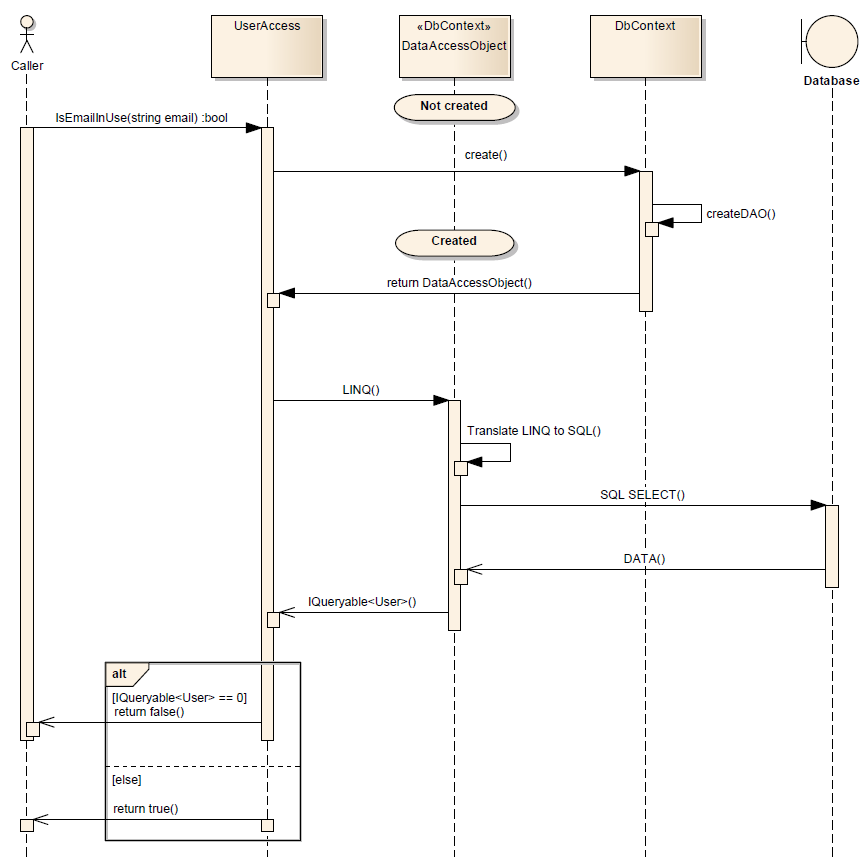
\includegraphics[width=\linewidth]{figs/dbSeq/isEmailInUse.PNG}
\caption{Sekvensdiagram for metoden IsEmailInUse}
\label{fig:isEmailInUse}
\end{figure}


\subparagraph{ValidatePassword}\

\textit{bool ValidatePassword(string email, string password)}

Når der er brug for at validere en brugers password, kaldes denne funktion. Den bruges eksempelvis når en bruger ønsker at logge ind på systemet. Se metodens sekvens diagram på figur~\ref{fig:validatePassword}.
	
\begin{figure}[h]
\centering
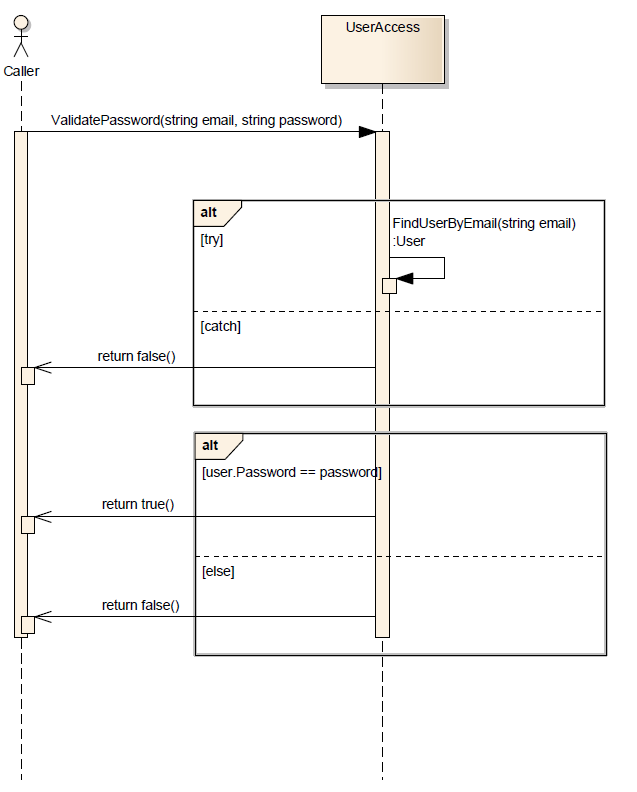
\includegraphics[width=0.7\linewidth]{figs/dbSeq/validatePassword.PNG}
\caption{Sekvensdiagram for metoden ValidatePassword}
\label{fig:validatePassword}
\end{figure}


\subparagraph{RemoveUser}\

\textit{void RemoveUser(string email)}

Checker først om en bruger med den bestemte email findes.
Laver en LINQ query på databasekontekst objektet, og finder den pågældende bruger.
Brugeren fjernes ved at kalde \textit{db.UserSet.Remove(user)} på kontekstobjektets UserSet property.

\begin{figure}[h]
\centering
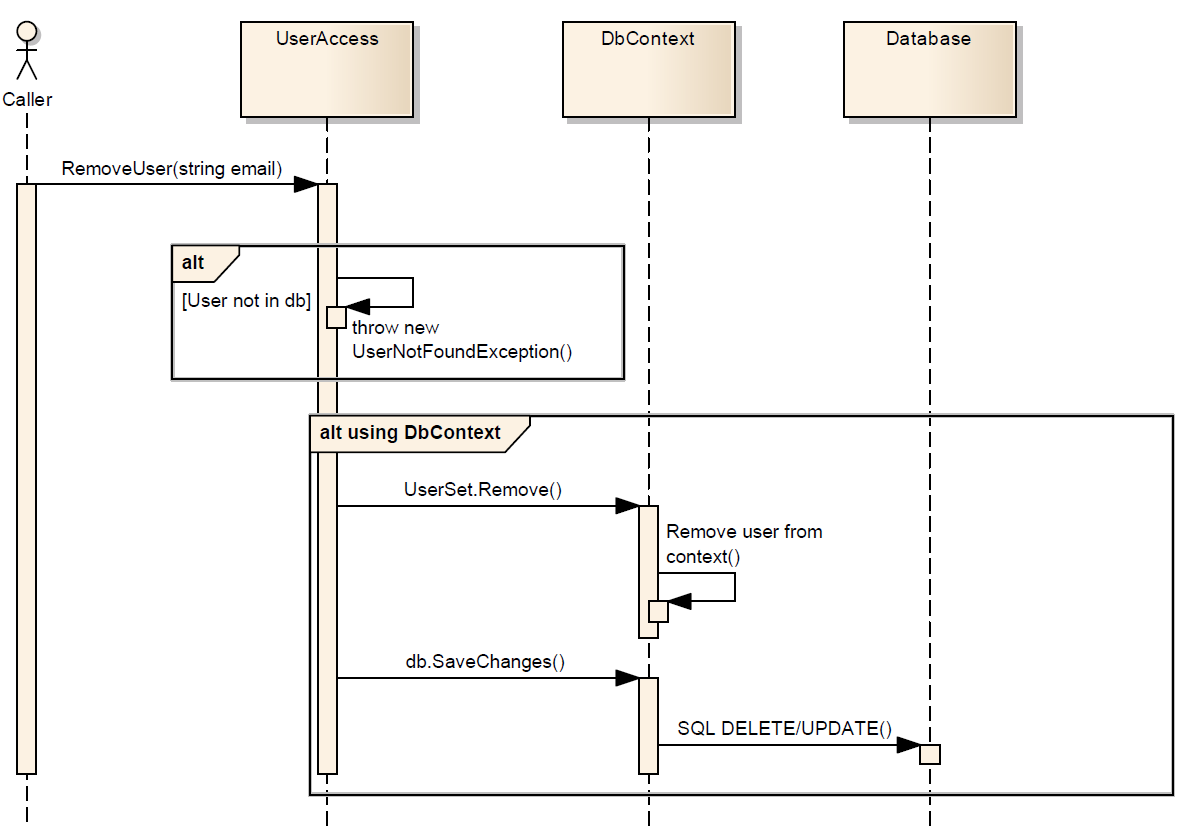
\includegraphics[width=\linewidth]{figs/dbSeq/removeUser.PNG}
\caption{Sekvensdiagram for metoden RemoveUser}
\label{fig:removeUser}
\end{figure}


\subparagraph{DeleteAllUsers}\

\textit{void DeleteAllUsers()}

Bruges kun under systemtest og udvikling.
Sletter alle brugere i databasen. Dette gøres ved at eksekvere en SQL kommando direkte på databasen. 

\begin{lstlisting}[caption=SQL injection på databasen ved sletning af brugere, label=sqlDeleteUsers]
...
using (var db = new DatabaseContext())
{
	db.Database.ExecuteSqlCommand("DELETE [UserSet]");
}
...	
\end{lstlisting}

\subparagraph{EditUserPassword}\

\textit{bool EditUserPassword(string email, string newPassword)}

Gør det muligt for en bruger at ændre sit password. Metoden står derudover for at sikre at det nye password ikke er en tom streng. User entitetens password property ændres gennem databasekonteksobjektet, hvorefter ændringen gemmes på databasen.
Metoden returnerer true med mindre der findes en uoverensstemmelse med enten password eller email.

\subparagraph{EditUserEmail}\

\textit{bool EditUserEmail(string email, string newEmail)}

Gør det muligt for en bruger at ændre sin email. Dette gøres gennem databasekontekst objektet. Når emailen er ændret skal brugeren benytte sig af den nye email ved et system login. \textit{Find()} metoden kaldes på kontekstobjektets UserSet property, med den ønskede brugers primærnøgle, \textit{Id}, hvorefter det pågældende User objekt returneres. Se kodeudsnit \ref{code:idef} for eksempel på brugen af primær nøgler i entity frameworket.

\begin{lstlisting}[caption=EditUserEmail - brug af primær nøgler i Entity Framework,label=code:idef]
public bool EditUserEmail(string email, string newEmail)
{
	...
	using (var db = new DatabaseContext())
	{
		var original = db.UserSet.Find(FindUserByEmail(email).Id);
		if (original != null)
			{
				original.Email = newEmail;
				db.SaveChanges();
			}
	}
	return true;
}

\end{lstlisting}

\subparagraph{EditUserName}\

\textit{bool EditUserName(string email, string newName)}
Selvom der ikke findes en user story der ønsker funktionalitet til at ændre en bruger/User's navn, er der skrevet ekstra funktionalitet dertil. Dette er gjort for at fremtidssikre data access laget.

Se sekvensdiagrammet på figur~\ref{fig:editUserName}

\begin{figure}[h]
\centering
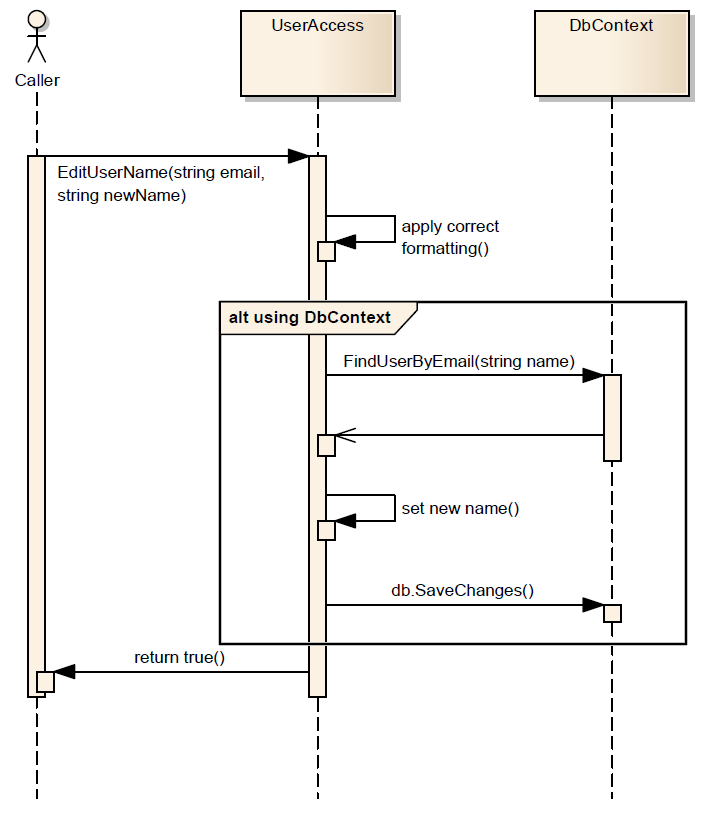
\includegraphics[width=0.7\linewidth]{figs/dbSeq/editUserName.PNG}
\caption{Sekvensdiagram for metoden EditUserName}
\label{fig:editUserName}
\end{figure}


\paragraph{Properties}\
\subsection{PoolAccess}
PoolAccess implementerer IPoolAccess og står for at skrive og læse pool records til/fra databasen. PoolAccess indeholder administrator funktionalitet vedligeholde pools i databasen. Herudover står PoolAcces for data redigering af pools samt validering af pooldata før de gemmes.

\begin{figure}
\centering
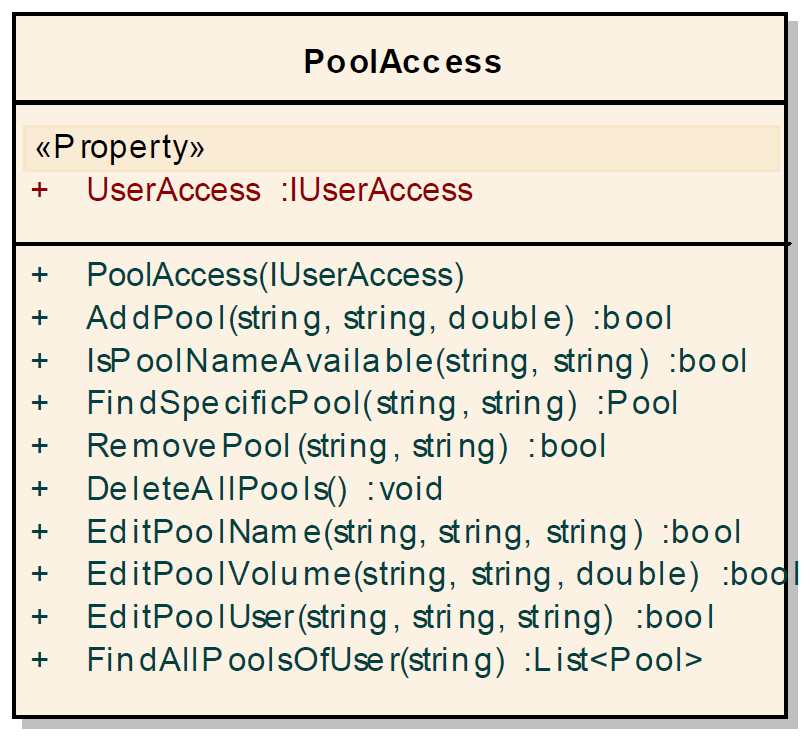
\includegraphics[width=0.46\linewidth]{figs/implementering/poolAccessClass.PNG}
\caption{Klassen PoolAccess.}
\label{fig:poolAccessClass}
\end{figure}

\subsubsection{AddPool}%%%%%%%%%%%%%%%%%%%%%%%%%%%%%%%%%%%%%%%%%%%%%%%%%%%%%%%%

\paragraph{Signatur}
\begin{itemize}
	\item \textit{bool AddPool(string email, string name, double volume)}
\end{itemize}

\paragraph{Returnere:}
\begin{itemize}
	\item \textit{Boolean}, true hvis poolen er sat ind i databasen uden problemer, ellers false.
\end{itemize}

\paragraph{Argumenter:}
\begin{enumerate}
	\item \textit{string} email addressen til den bruger som poolen skal tildeles.
	\item \textit{string} navnet som brugeren vil bruge til at identificere poolen.
	\item \textit{string} poolens volume i $m^3$.
\end{enumerate}

\paragraph{Virkemåde}
\begin{itemize}
	\item Metoden tjekker først om brugeren allerede har oprettet en pool med det sammen navn, hvis dette er tilfældet vil metoden returnere \textit{false}. Metoden sikre også at poolens navn ikke er tomt. Hvis brugeren ikke har en pool med samme navn, vil poolen bliver oprettet i databasen.
\end{itemize}

\subsubsection{IsPoolNameAvailable}%%%%%%%%%%%%%%%%%%%%%%%%%%%%%%%%%%%%%%%%%%%%%%%%%%%%%%%%






\paragraph{Signatur}
\begin{itemize}
	\item \textit{bool IsPoolNameAvailable(string email, string name)}
\end{itemize}

\paragraph{Returnere:}
\begin{itemize}
	\item \textit{Boolean}, true hvis navnet er ledigt og false hvis det er taget. To brugere kan godt begge have en pool med det samme navn.
\end{itemize}

\paragraph{Argumenter:}
\begin{enumerate}
	\item \textit{string} email addressen til den bruger som har poolen.
	\item \textit{string} navnet som brugeren har valgt til at identificere poolen.
\end{enumerate}

\paragraph{Virkemåde}
\begin{itemize}
	\item Metoden finder alle pools i databasen som har dette navn. Derefter tjekker den om en af disse pool tilhører brugeren, ved hjælp af email addressen.
\end{itemize}









\subsubsection{FindSpecificPool}%%%%%%%%%%%%%%%%%%%%%%%%%%%%%%%%%%%%%%%%%%%%%%%%%%%%%%%%





\paragraph{Signatur}
\begin{itemize}
	\item \textit{Pool FindSpecificPool(string email, string name)}
\end{itemize}

\paragraph{Returnere:}
\begin{itemize}
	\item \textit{Pool} en instans af pool objektet, som har samme attributter som poolen i databasen.
\end{itemize}

\paragraph{Argumenter:}
\begin{enumerate}
	\item \textit{string} email addressen til den bruger som har poolen.
	\item \textit{string} navnet som brugeren har valgt til at identificere poolen med.
\end{enumerate}

\paragraph{Virkemåde}
\begin{itemize}
	\item Metoden tjekker først om den valgte kombination af email og navn findes i databasen. Hvis kombinationen findes, henter den poolen og returnere denne.
\end{itemize}








\subsubsection{RemovePool}%%%%%%%%%%%%%%%%%%%%%%%%%%%%%%%%%%%%%%%%%%%%%%%%%%%%%%%%

\paragraph{Signatur}
\begin{itemize}
	\item \textit{bool RemovePool(string email, string name)}
\end{itemize}

\paragraph{Returnere:}
\begin{itemize}
	\item \textit{Boolean}, true hvis poolen kunne fjernes fra databasen uden problemer, false ved fejl.
\end{itemize}

\paragraph{Argumenter:}
\begin{enumerate}
	\item \textit{string} email addressen til den bruger som har poolen.
	\item \textit{string} navnet som brugeren har valgt til at identificere poolen med.
\end{enumerate}

\paragraph{Virkemåde}
\begin{itemize}
	\item Metoden tjekker først om den valgte kombination af email og navn findes i databasen. Hvis kombinationen findes, henter den poolen ved navn og hvis det er brugerens pool bliver den fjernet.
\end{itemize}

\subsubsection{DeleteAllPools}%%%%%%%%%%%%%%%%%%%%%%%%%%%%%%%%%%%%%%%%%%%%%%%%%%%%%%%%




\paragraph{Signatur}
\begin{itemize}
	\item \textit{void DeleteAllPools()}
\end{itemize}

\paragraph{Returnere:}
\begin{itemize}
	\item \textit{void}.
\end{itemize}

\paragraph{Argumenter:}
\begin{enumerate}
	\item Tager ikke nogle argumenter.
\end{enumerate}

\paragraph{Virkemåde}
\begin{itemize}
	\item Metoden er lavet til brug under udvikling og test. Den fjerner alle pools i databasen.
\end{itemize}






\subsubsection{EditPoolName}%%%%%%%%%%%%%%%%%%%%%%%%%%%%%%%%%%%%%%%%%%%%%%%%%%%%%%%%





\paragraph{Signatur}
\begin{itemize}
	\item \textit{bool EditPoolName(string ownerEmail, string currentName, string newName)}
\end{itemize}

\paragraph{Returnere:}
\begin{itemize}
	\item \textit{Boolean}, true hvis poolen attributter kunne ændres uden fejl, ellers false.
\end{itemize}

\paragraph{Argumenter:}
\begin{enumerate}
	\item \textit{string} email addressen til den bruger som har poolen.
	\item \textit{string} navnet som brugeren har valgt til at identificere poolen med.
	\item \textit{string} det nye navn som pool skal tildeles.
\end{enumerate}

\paragraph{Virkemåde}
\begin{itemize}
	\item Metoden tjekker først om det nye navn er gyldigt (ikke en tom string). Så tjekkes det om den valgte kombination af email og navn findes i databasen. Hvis kombinationen findes, henter den poolen ved navn og hvis det er brugerens pool bliver navnet ændret.
\end{itemize}





\subsubsection{EditPoolVolume}%%%%%%%%%%%%%%%%%%%%%%%%%%%%%%%%%%%%%%%%%%%%%%%%%%%%%%%%







\paragraph{Signatur}
\begin{itemize}
	\item \textit{bool EditPoolVolume(string ownerEmail, string name, double newVolume)}
\end{itemize}

\paragraph{Returnere:}
\begin{itemize}
	\item \textit{Boolean}, true hvis poolen attributter kunne ændres uden fejl, ellers false.
\end{itemize}

\paragraph{Argumenter:}
\begin{enumerate}
	\item \textit{string} email addressen til den bruger som har poolen.
	\item \textit{string} navnet som brugeren har valgt til at identificere poolen med.
	\item \textit{double} det nye volumen som pool skal tildeles.
\end{enumerate}

\paragraph{Virkemåde}
\begin{itemize}
	\item Metoden tjekker først om det nye volume er gyldigt (ikke en tom string). Så tjekkes det om den valgte kombination af email og navn findes i databasen. Hvis kombinationen findes, henter den poolen ved navn og hvis det er brugerens pool bliver navnet ændret.
\end{itemize}





\subsubsection{EditPoolUser}%%%%%%%%%%%%%%%%%%%%%%%%%%%%%%%%%%%%%%%%%%%%%%%%%%%%%%%%







\paragraph{Signatur}
\begin{itemize}
	\item \textit{bool EditPoolUser(string currectOwnerEmail, string name, string newUserEmail)}
\end{itemize}

\paragraph{Returnere:}
\begin{itemize}
	\item \textit{Boolean}, true hvis poolen kunne fjernes fra tidligere bruger til tilføjes den nye, ellers false.
\end{itemize}

\paragraph{Argumenter:}
\begin{enumerate}
	\item \textit{string} email addressen til den bruger som har poolen.
	\item \textit{string} navnet som brugeren har valgt til at identificere poolen med.
	\item \textit{string} email addressen til den nye bruger som skal have poolen.
\end{enumerate}

\paragraph{Virkemåde}
\begin{itemize}
	\item Metoden tjekker først om den valgte kombination af email og navn findes i databasen. Hvis kombinationen findes, testes det om den nye bruger eksistere. Hvis den nye bruger ikke allerede har en pool med samme navn, bliver poolen fjernet fra den gamle bruger og tilføjet den nye.
\end{itemize}






\subsubsection{FindAllPoolsOfUser}%%%%%%%%%%%%%%%%%%%%%%%%%%%%%%%%%%%%%%%%%%%%%%%%%%%%%%%%








\paragraph{Signatur}
\begin{itemize}
	\item \textit{List<Pool> FindAllPoolsOfUser(string ownerEmail}
\end{itemize}

\paragraph{Returnere:}
\begin{itemize}
	\item \textit{List<Pool>}, som indeholder alle pool tilknyttet en bruger.
\end{itemize}

\paragraph{Argumenter:}
\begin{enumerate}
	\item \textit{string} email addressen til den bruger, som pools skal findes for.
\end{enumerate}

\paragraph{Virkemåde}
\begin{itemize}
	\item Først tester metoden om brugeren findes i databasen, hvis denne ikke kan findes smides en \textit{UserNotFoundException()}. Dernæst findes alle pools med tilknytning til brugeren og disse returneres.
\end{itemize}






\subsubsection{UserAccess}%%%%%%%%%%%%%%%%%%%%%%%%%%%%%%%%%%%%%%%%%%%%%%%%%%%%%%%%

\textit{IUserAccess UserAccess { get; set; }}
\subsubsection{Klassen DataAccess}
DataAccess implementerer IDataAccess og står for at skrive og læse data records til/fra databasen.
IDataAccess refereres af klassen SmartPoolDB. Klassen DataAccess kan ses på figur \ref{fig:dataAccessClassNoInherit}

\begin{figure}[H]
\centering
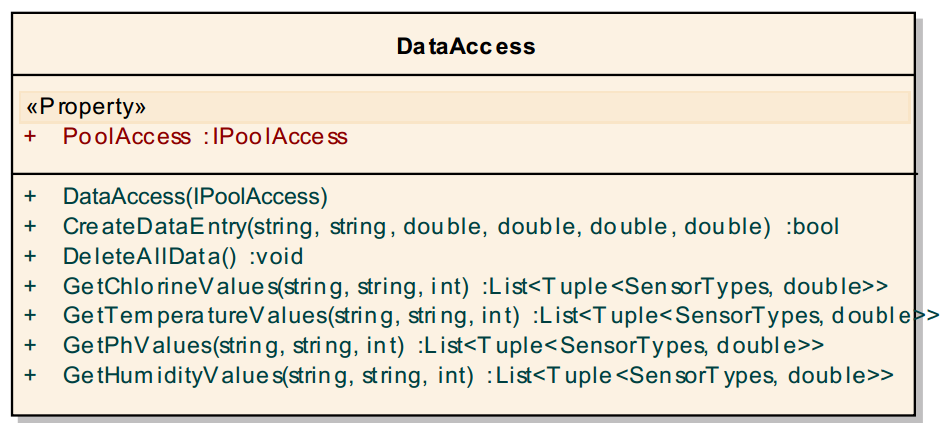
\includegraphics[width=0.7\linewidth]{figs/dbExtra/classdiadata.png}
\caption{Klassediagram for DataAccess}
\label{fig:classdiadata}
\end{figure}


\begin{figure}[h]
\centering
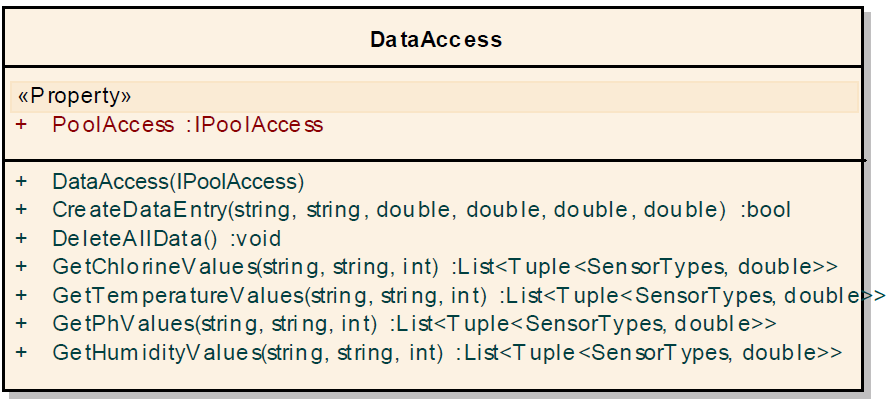
\includegraphics[width=0.7\linewidth]{figs/implementering/dataAccessClassNoInherit}
\caption{Klassen DataAccess}
\label{fig:dataAccessClassNoInherit}
\end{figure}

\paragraph{CreateDataEntry}\ %%%%%%%%%%%%%%%%%%%%%%%%%%%%%%%%%%%%%%%%%%%%%%%%%%%%%%%%%%%%%%%%%%%

\subparagraph{Signatur}
\begin{itemize}
	\item \textit{bool CreateDataEntry(string ownerEmail, string poolName, double chlorine, double temp, double pH, double humidity)}
\end{itemize}

\subparagraph{Returnerer:}
\begin{itemize}
	\item \textit{Boolean}, true hvis data kunne sættes ind i databasen uden problemer, ellers false.
\end{itemize}

\subparagraph{Argumenter:}
\begin{enumerate}
	\item \textit{string} email addressen til den bruger, som poolen tilhører.
	\item \textit{string} navnet på poolen.
	\item \textit{double} klor værdien som skal indsættes.
	\item \textit{double} temperatur værdien som skal indsættes.
	\item \textit{double} pH værdien som skal indsættes.
	\item \textit{double} luftfugtigheds værdien som skal indsættes.
\end{enumerate}

\subparagraph{Virkemåde}

\begin{itemize}
	\item Først tester metoden om brugeren har en pool med det givne navn. Metoden gemmer så tidspunktet og opretter et \textit{Data} object (som vist i figur~\ref{fig:datasetentity}), som gemmes i databasen. Herefter oprettes målingerne og tildeles den fælles \textit{Data} som tidligere blev oprettet. Se metodens sekvensdiagram på figur~\ref{fig:EFarch}
\end{itemize}

\begin{figure}[h]
\centering
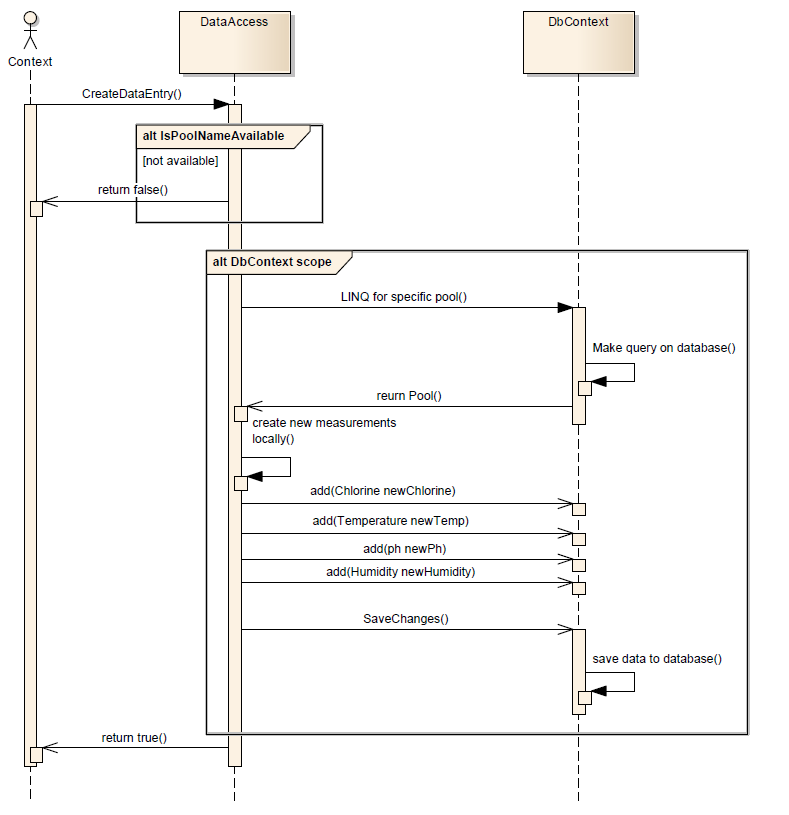
\includegraphics[width=0.7\linewidth]{figs/dbSeq/createDataEntry.PNG}
\caption{Sekvensdiagram for metoden CreateDataEntry}
\label{fig:createDataEntry}
\end{figure}

\begin{figure}[h]
\centering
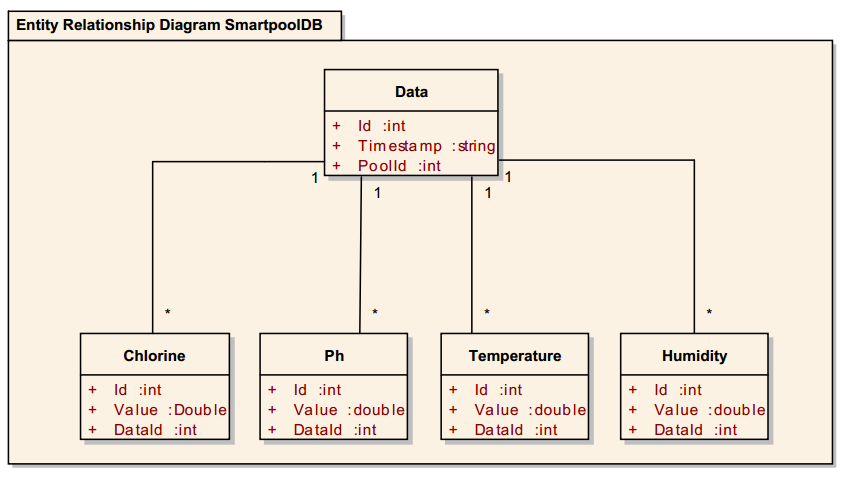
\includegraphics[width=0.8\linewidth]{figs/implementering/datasetentity.png}
\caption{En del af ER diagrammet som databasen er lavet udfra.}
\label{fig:datasetentity}
\end{figure}

\paragraph{DeleteAllData}\ %%%%%%%%%%%%%%%%%%%%%%%%%%%%%%%%%%%%%%%%%%%%%%%%%%%%%%%%%%%%%%%%%%%

\subparagraph{Signatur}
\begin{itemize}
	\item \textit{void DeleteAllData()}
\end{itemize}

\subparagraph{Returnerer:}
\begin{itemize}
	\item \textit{void}.
\end{itemize}

\subparagraph{Argumenter:}
\begin{enumerate}
	\item Tager ikke nogle argumenter.
\end{enumerate}

\subparagraph{Virkemåde}
\begin{itemize}
	\item Lavet til brug under test og udvikling. Rydder tabellerne for Data og målinger (Chlorine, Ph...).
\end{itemize}


\paragraph{GetChlorineValues}\ %%%%%%%%%%%%%%%%%%%%%%%%%%%%%%%%%%%%%%%%%%%%%%%%%%%%%%%%%%%%%%%%%%%


\subparagraph{Signatur}
\begin{itemize}
	\item \textit{List<Tuple<SensorTypes, double>> GetChlorineValues(string poolOwnerEmail, string poolName, int daysToGoBack)}
\end{itemize}

\subparagraph{Returnerer:}
\begin{itemize}
	\item \textit{List<Tuple<SensorTypes, double>>} - \textit{SensorTypes} er et enum for typen af måler/sensor (klor for denne metode), \textit{double} er den målte værdi. Disse bliver returneret i en \textit{Tuple} og alle målinger lavet i det valgte tidsrum bliver lagt ind i listen.
\end{itemize}

\subparagraph{Argumenter:}
\begin{enumerate}
	\item \textit{string} email addressen til den bruger, som poolen tilhøre.
	\item \textit{string} navnet på poolen.
	\item \textit{int} hvor langt tilbage der skal findes målinger for. Eksempelvis vil $daysToGoBack == 2$ finde alle målinger foretaget indenfor de sidste 48 timer.
\end{enumerate}

\subparagraph{Virkemåde}
\begin{itemize}
	\item Metoden laver først \textit{daysToGoBack} om til \textit{DateTime}-format. Så beregnes \textit{DateTime} for tidspunktet som der skal gås tilbage til. Så findes alle klor-målinger og endeligt fravælges alle som ikke ligge i det rigtige tidsrum. Se metodens sekvensdiagram på figur~\ref{fig:getChlorineData}
\end{itemize}

\begin{figure}[h]
\centering
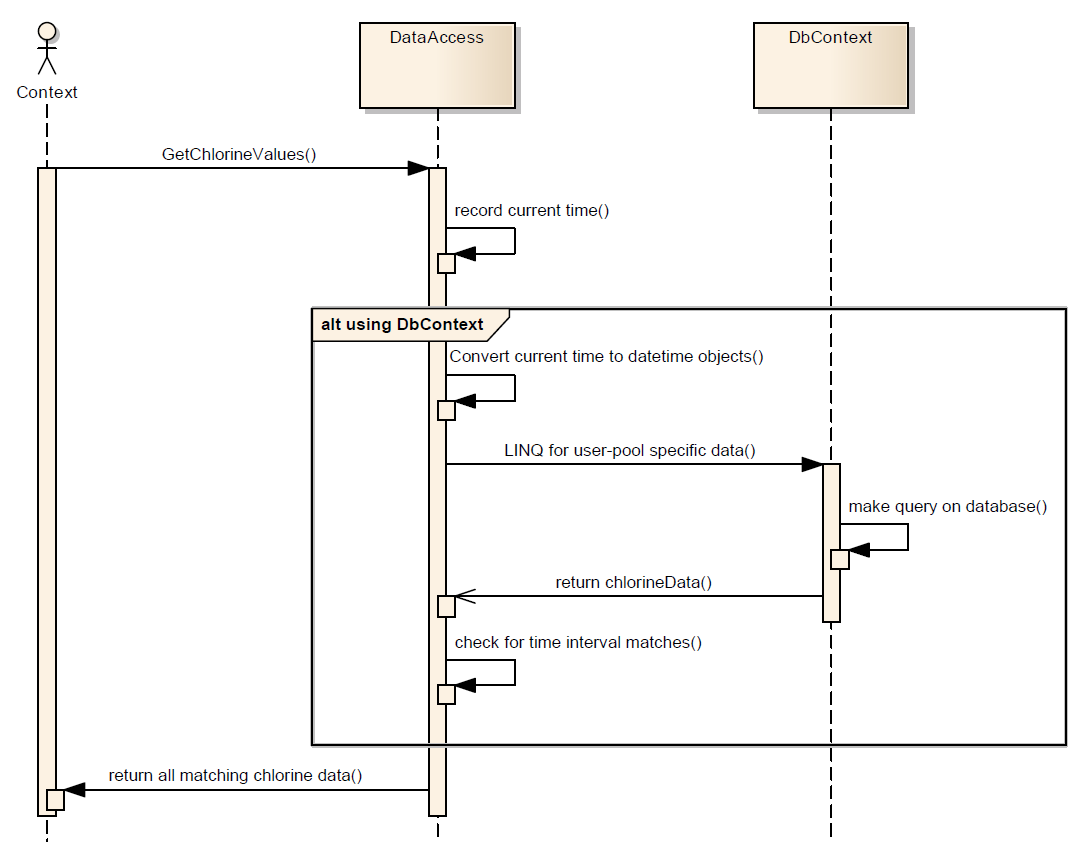
\includegraphics[width=0.7\linewidth]{figs/dbSeq/getChlorineData.PNG}
\caption{Sekvensdiagram for metoden GetChlorineData}
\label{fig:getChlorineData}
\end{figure}


\subparagraph{GetTemperatureValues}\ %%%%%%%%%%%%%%%%%%%%%%%%%%%%%%%%%%%%%%%%%%%%%%%%%%%%%%%%%%%%%%%%%%%


\subparagraph{Signatur}
\begin{itemize}
	\item \textit{List<Tuple<SensorTypes, double>> GetTemperatureValues(string poolOwnerEmail, string poolName, int daysToGoBack)}
\end{itemize}

\subparagraph{Returnerer:}
\begin{itemize}
	\item \textit{List<Tuple<SensorTypes, double>>} - \textit{SensorTypes} er et enum for typen af måler/sensor (temperatur for denne metode), \textit{double} er den målte værdi. Disse bliver returneret i en \textit{Tuple} og alle målinger lavet i det valgte tidsrum bliver lagt ind i listen.
\end{itemize}

\subparagraph{Argumenter:}
\begin{enumerate}
	\item \textit{string} email addressen til den bruger, som poolen tilhøre.
	\item \textit{string} navnet på poolen.
	\item \textit{int} hvor langt tilbage der skal findes målinger for. Eksempelvis vil $daysToGoBack == 2$ finde alle målinger foretaget indenfor de sidste 48 timer.
\end{enumerate}

\subparagraph{Virkemåde}
\begin{itemize}
	\item Metoden laver først \textit{daysToGoBack} om til \textit{DateTime}-format. Så beregnes \textit{DateTime} for tidspunktet som der skal gås tilbage til. Så findes alle temperatur-målinger og endeligt fravælges alle som ikke ligge i det rigtige tidsrum. Se evt. sekvensdiagrammet for \textit{GetChlorineData} på figur~\ref{fig:getChlorineData}, da funktionaliteten er den samme.
\end{itemize}


\subparagraph{GetPhValues}\ %%%%%%%%%%%%%%%%%%%%%%%%%%%%%%%%%%%%%%%%%%%%%%%%%%%%%%%%%%%%%%%%%%%

\textit{List<Tuple<SensorTypes, double>> GetPhValues(string poolOwnerEmail, string poolName, int daysToGoBack)}


\subparagraph{Signatur}
\begin{itemize}
	\item \textit{List<Tuple<SensorTypes, double>> GetPhValues(string poolOwnerEmail, string poolName, int daysToGoBack)}
\end{itemize}

\subparagraph{Returnerer:}
\begin{itemize}
	\item \textit{List<Tuple<SensorTypes, double>>} - \textit{SensorTypes} er et enum for typen af måler/sensor (pH for denne metode), \textit{double} er den målte værdi. Disse bliver returneret i en \textit{Tuple} og alle målinger lavet i det valgte tidsrum bliver lagt ind i listen.
\end{itemize}

\subparagraph{Argumenter:}
\begin{enumerate}
	\item \textit{string} email addressen til den bruger, som poolen tilhøre.
	\item \textit{string} navnet på poolen.
	\item \textit{int} hvor langt tilbage der skal findes målinger for. Eksempelvis vil $daysToGoBack == 2$ finde alle målinger foretaget indenfor de sidste 48 timer.
\end{enumerate}

\subparagraph{Virkemåde}
\begin{itemize}
	\item Metoden laver først \textit{daysToGoBack} om til \textit{DateTime}-format. Så beregnes \textit{DateTime} for tidspunktet som der skal gås tilbage til. Så findes alle pH-målinger og endeligt fravælges alle som ikke ligge i det rigtige tidsrum. Se evt. sekvensdiagrammet for \textit{GetChlorineData} på figur~\ref{fig:getChlorineData}, da funktionaliteten er den samme.
\end{itemize}

\subparagraph{GetHumidityValues}\ %%%%%%%%%%%%%%%%%%%%%%%%%%%%%%%%%%%%%%%%%%%%%%%%%%%%%%%%%%%%%%%%%%%

\subparagraph{Signatur}
\begin{itemize}
	\item \textit{List<Tuple<SensorTypes, double>> GetHumidityValues(string poolOwnerEmail, string poolName, int daysToGoBack);}
\end{itemize}

\subparagraph{Returnerer:}
\begin{itemize}
	\item \textit{List<Tuple<SensorTypes, double>>} - \textit{SensorTypes} er et enum for typen af måler/sensor (luftfugtighed for denne metode), \textit{double} er den målte værdi. Disse bliver returneret i en \textit{Tuple} og alle målinger lavet i det valgte tidsrum bliver lagt ind i listen.
\end{itemize}

\subparagraph{Argumenter:}
\begin{enumerate}
	\item \textit{string} email addressen til den bruger, som poolen tilhøre.
	\item \textit{string} navnet på poolen.
	\item \textit{int} hvor langt tilbage der skal findes målinger for. Eksempelvis vil $daysToGoBack == 2$ finde alle målinger foretaget indenfor de sidste 48 timer.
\end{enumerate}

\subparagraph{Virkemåde}
\begin{itemize}
	\item Metoden laver først \textit{daysToGoBack} om til \textit{DateTime}-format. Så beregnes \textit{DateTime} for tidspunktet som der skal gås tilbage til. Så findes alle luftfugtigheds-målinger og endeligt fravælges alle som ikke ligge i det rigtige tidsrum. Se evt. sekvensdiagrammet for \textit{GetChlorineData} på figur~\ref{fig:getChlorineData}, da funktionaliteten er den samme.
\end{itemize}


